%!TEX root = ../paper.tex

\section{Introduction}
\label{sec:introduction}

% TODO Figure 1

Due to the immense growth of the internet and the blogosphere, users have an overwhelming amount of potential reading material available.
Since maintaining a blog requires very little technical knowledge, nearly anyone can write a blog on any number of topics.
This poses a problem for the reader as there is a gigantic number of different blogs available and only very basic discovery mechanisms are in place.


Since people often have distinctive writing styles, these could allow for a topic-independent classification of blog authors.
Such a classification would allow readers of one blog to find other, similarly written blogs, which might be interesting to them.
The fact that writing styles are topic-independent can be advantageous for blog classification for multiple reasons: It would enable us to find other blogs of an author for which he uses a different alias.
Additionally, readers could find blogs with a similar writing style to that of an author they enjoy reading and then filter for topics they are interested in, even if they are entirely unrelated to the original author's topics.
Furthermore, such a system could be used to help identify authors for individual blog posts where the author information is not available.
Advanced scenarios from the security domain might be trying to find the author of a piece of leaked information or of overly inflammatory or defamatory blogs.


One of the main issues in designing a classification program of this kind is the pure scale of the problem when regarding the blogosphere as a whole.
Being able to distinguish tens or even hundreds of thousands of authors purely by their writing style is much harder than it would be for only a few dozen authors.
Reliably finding the one matching author on this scale might, in fact, be impossible with today's methods.
Instead, we aimed to create a program which should output a number of blogs with a writing style similar to that of a given document.


To that end, we first extract a number of significant features (Section~\ref{sec:features}) - such as lexical diversity or the use of certain function words - from each blog post which are relevant in determining the writing style.
Then, we use a clustering step to group blog posts with similar writing styles together (Section~\ref{sec:k-means}), based on their features.
The resulting clusters are then labelled according to their most distinctive shared features (Section~\ref{sec:cluster_labeling}), to allow the users to see what its containing documents have in common.
A model generated from these clusters is then fed to a machine learning step (Section~\ref{sec:classification}) which is able to discern the cluster a given new document would belong to.
To this end, the features of the new document are calculated and then compared to the model of known documents and their clusters.


\begin{figure}[h]
    \centering
    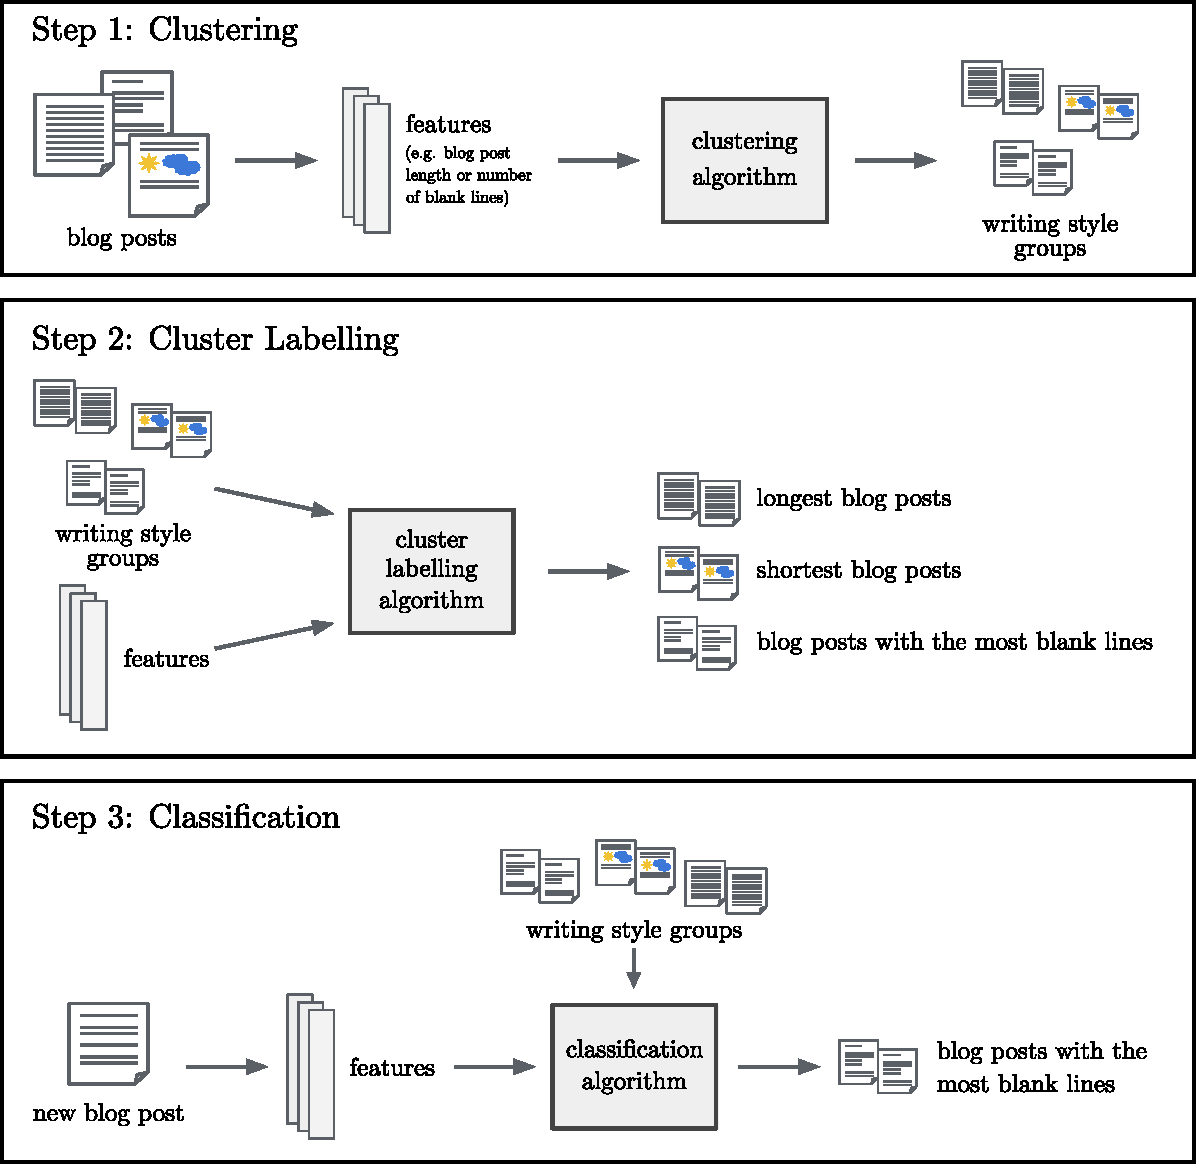
\includegraphics[width=0.8\textwidth]{images/Figure_1.pdf}
    \caption{}
    \label{fig:naive}
\end{figure}


Since many of the features which discern a writing style are not comparable across different languages (e.g. the average word length might be vastly different between various languages, making it useless when comparing an English post to a French one), we decided to focus on only two languages: English and German.
For the reason mentioned above, our program will still only work with one of these languages at a time but it can function with documents from either of them.